%!TEX program = xelatex
\documentclass[12pt, a4paper]{article}

\usepackage[dvipsnames]{xcolor}

\usepackage{fancyhdr}
\usepackage{extramarks}
\usepackage{amsmath}
\usepackage{amsthm}
\usepackage{amsfonts}
\usepackage{tikz}
\usepackage[plain]{algorithm}
\usepackage{algpseudocode}

\usepackage{ctex}
\usepackage{indentfirst}
\usepackage{wrapfig}
\usepackage{upgreek}
\usepackage{subfigure}
\ctexset {today=old}
\usetikzlibrary{automata,positioning,shapes.geometric,arrows.meta,patterns,calc}
\numberwithin{equation}{section}

%
% Basic Document Settings
%

\topmargin=-0.25in
\evensidemargin=0in
\oddsidemargin=0in
\textwidth=6.5in
\textheight=9.2in
\headsep=0.25in

\linespread{1.1}

\pagestyle{fancy}
\lhead{\hmwkAuthorName}
\chead{\hmwkClass : \hmwkTitle}
\rhead{\firstxmark}
\lfoot{\lastxmark}
\cfoot{\thepage}

\renewcommand\headrulewidth{0.4pt}
\renewcommand\footrulewidth{0.4pt}

\setlength{\parindent}{2em}  % 2em代表首行缩进两个字符

%
% Create Problem Sections
%

\newcommand{\enterProblemHeader}[1]{
    \nobreak\extramarks{}{Problem \arabic{#1} continued on next page\ldots}\nobreak{}
    \nobreak\extramarks{Problem \arabic{#1} (continued)}{Problem \arabic{#1} continued on next page\ldots}\nobreak{}
}

\newcommand{\exitProblemHeader}[1]{
    \nobreak\extramarks{Problem \arabic{#1} (continued)}{Problem \arabic{#1} continued on next page\ldots}\nobreak{}
    \stepcounter{#1}
    \nobreak\extramarks{Problem \arabic{#1}}{}\nobreak{}
}

% \setcounter{secnumdepth}{0}
\newcounter{partCounter}
\newcounter{homeworkProblemCounter}
\setcounter{homeworkProblemCounter}{0}
% \nobreak\extramarks{Problem \arabic{homeworkProblemCounter}}{}\nobreak{}

%
% Homework Problem Environment
%
% This environment takes an optional argument. When given, it will adjust the
% problem counter. This is useful for when the problems given for your
% assignment aren't sequential. See the last 3 problems of this template for an
% example.
%
\newenvironment{homeworkProblem}[1][-1]{
    \ifnum#1>0
        \setcounter{homeworkProblemCounter}{#1}
    \fi
    \section{Problem \arabic{homeworkProblemCounter}}
    \setcounter{partCounter}{1}
    \enterProblemHeader{homeworkProblemCounter}
}{
    \exitProblemHeader{homeworkProblemCounter}
}

%
% Homework Details
%   - Title
%   - Due date
%   - Class
%   - Section/Time
%   - Instructor
%   - Author
%

\newcommand{\hmwkTitle}{Rigid Body Mechanics}
\newcommand{\hmwkDueDate}{\today}
\newcommand{\hmwkClass}{University Physics}
\newcommand{\hmwkClassTime}{}
\newcommand{\myUniversiy}{Wuhan University}
\newcommand{\hmwkAuthorName}{\textbf{Lai Wei}}

%
% Title Page
%

\title{
    \vspace{2in}
    \textmd{\textbf{\hmwkClass:\ \hmwkTitle}}\\
    \normalsize\vspace{0.1in}\small{Date: \hmwkDueDate}\\
    \vspace{0.1in}\large{\textit{\myUniversiy}}
    \vspace{3in}
}

\author{\hmwkAuthorName}
\date{}

\renewcommand{\part}[1]{\textbf{\large Part \Alph{partCounter}}\stepcounter{partCounter}\\}

%
% Various Helper Commands
%

% Useful for algorithms
\newcommand{\alg}[1]{\textsc{\bfseries \footnotesize #1}}

% % For derivatives
% \newcommand{\deriv}[1]{\frac{\mathrm{d}}{\mathrm{d}x} (#1)}

% For partial derivatives
\newcommand{\pderiv}[2]{\frac{\partial}{\partial #1} (#2)}

% Integral dx
\newcommand{\dx}{\mathrm{d}x}

% Alias for the Solution section header
\newcommand{\solution}{\textbf{\large Solution}}

% Probability commands: Expectation, Variance, Covariance, Bias
\newcommand{\E}{\mathrm{E}}
\newcommand{\Var}{\mathrm{Var}}
\newcommand{\Cov}{\mathrm{Cov}}
\newcommand{\Bias}{\mathrm{Bias}}

% 我的newcommand
\newcommand{\degree}{^{\circ}}
\newcommand{\arrow}{-{Stealth[length=4mm,width=2mm]}}
\newcommand{\rmd}{\mathrm{~d}}
\newcommand{\deriv}[2]{\frac{\rmd #1}{\rmd #2}}
\renewcommand{\parallel}{\mathrel{/\mskip-2.5mu/}}

\begin{document}

\maketitle

\pagebreak

% 设置页码格式是罗马数字
\pagenumbering{roman}

% 生成目录
\tableofcontents

\pagebreak

% 设置页码格式是阿拉伯数字
\pagenumbering{arabic}

\pagebreak

\section{刚体的定轴转动}

\subsection{刚体}

\subsubsection{定义}

    在外力作用下,形状和大小都不发生变化的物体。(任意两质点间距离保持不变的特殊质点组。)

    \begin{enumerate}
        \item 刚体是理想模型;
        \item 刚体模型是为简化研究问题而引进的。
    \end{enumerate}

\subsubsection{平动}

    刚体中所有点的运动轨迹都保持完全相同。(各点的状态一样)

    刚体上任意一点的运动可以代表整个刚体的运动。(刚体平动的运动规律和与质点的运动规律相同)

\subsection{转动}

    分为\textbf{定轴转动}和\textbf{非定轴转动}。

    刚体的一般运动可以看作“随质心的平动”和“绕质心的转动”的合成。

\subsubsection{刚体转动的角速度和角加速度}

    \begin{wrapfigure}{r}{4cm}
        \centering
        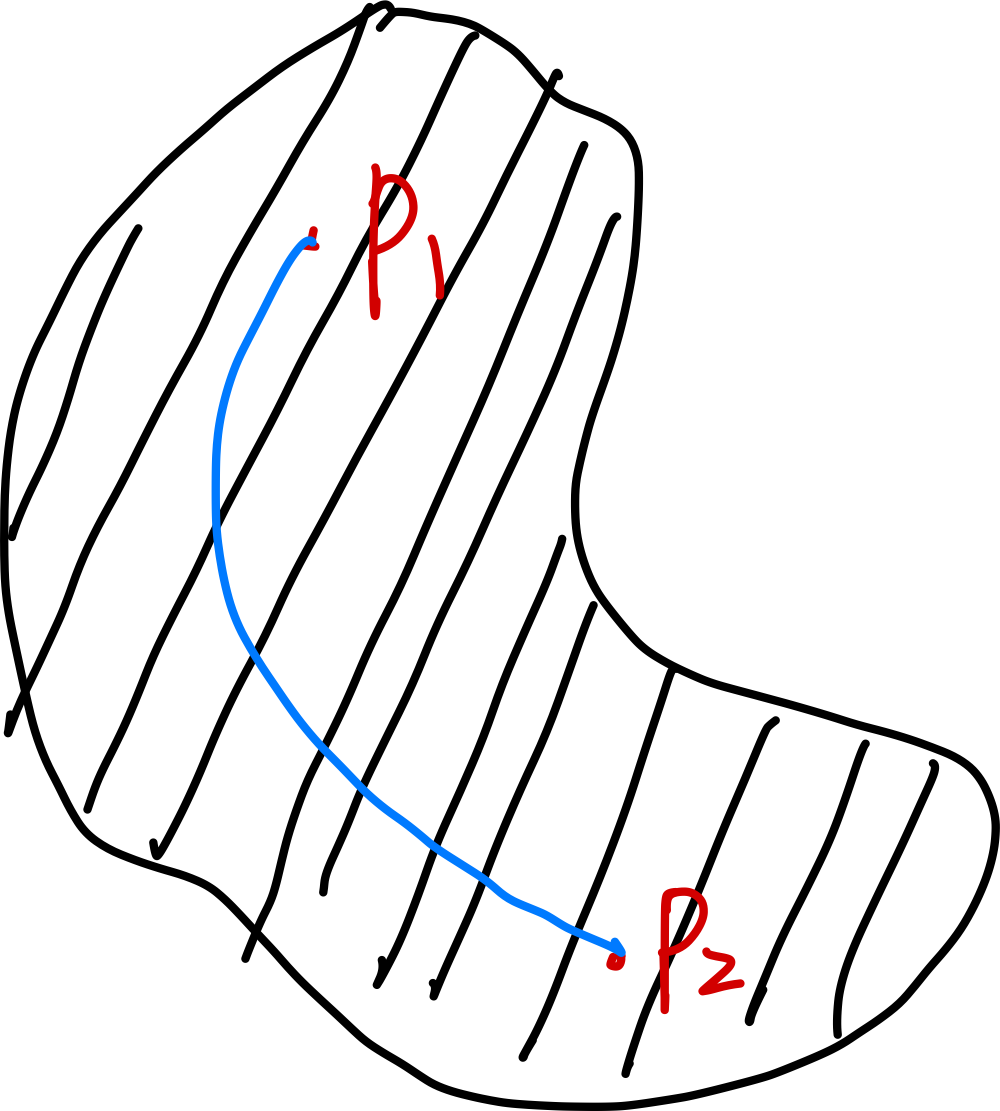
\includegraphics[scale=0.15]{"Chapter 04 images/pic1.png"}
        % \caption{}
        \label{pic4-1}
    \end{wrapfigure}

    角坐标\(\theta = \theta\left(t\right)\),沿逆时针方向转动为\(\theta > 0\),
    角位移\(\Delta \theta = \theta \left(t + \Delta t\right) - \theta\left(t\right)\)。
    角速度矢量

    \begin{equation}
        \omega=\lim _{\Delta t \rightarrow 0} \frac{\Delta \theta}{\Delta t}=\frac{\mathrm{d} \theta}{\mathrm{~d} t}
    \end{equation}

    方向按右手螺旋法则确定。

\subsubsection{刚体定轴转动}

    刚体定轴转动(一维转动)的转动方向可以用角速度的正、负来表示。

    角加速度

    $$
        \overrightarrow{\alpha} = \deriv{\overrightarrow{\omega}}{t}
    $$

    定轴转动的特点:

    \begin{enumerate}
        \item 每一质点均做圆周运动,与轴垂直的圆面为转动平面;
        \item 任意质点运动\(\Delta \theta,\; \omega,\; \overrightarrow{\omega},\; \overrightarrow{\alpha}\)相同,但\(\overrightarrow{v},\; \overrightarrow{a}\)不相同;
        \item 运动描述仅需一个坐标。
    \end{enumerate}

    匀变速转动公式:

    $$
    \begin{array}{|l|l|}
    \hline \text { 质点匀变速直线运动 } & \text { 刚体绕定轴匀变速转动 } \\
    \hline v=v_0+a t & \omega=\omega_0+\alpha t \\
    \hline x=x_0+v_0 t+\frac{1}{2} a t^2 & \theta=\theta_0+\omega_0 t+\frac{1}{2} \alpha t^2 \\
    \hline v^2=v_0^2+2 a\left(x-x_0\right) & \omega^2=\omega_0^2+2 \alpha\left(\theta-\theta_0\right) \\
    \hline
    \end{array}
    $$

    角量与线量的关系:

    \begin{wrapfigure}{r}{4cm}
        \centering
        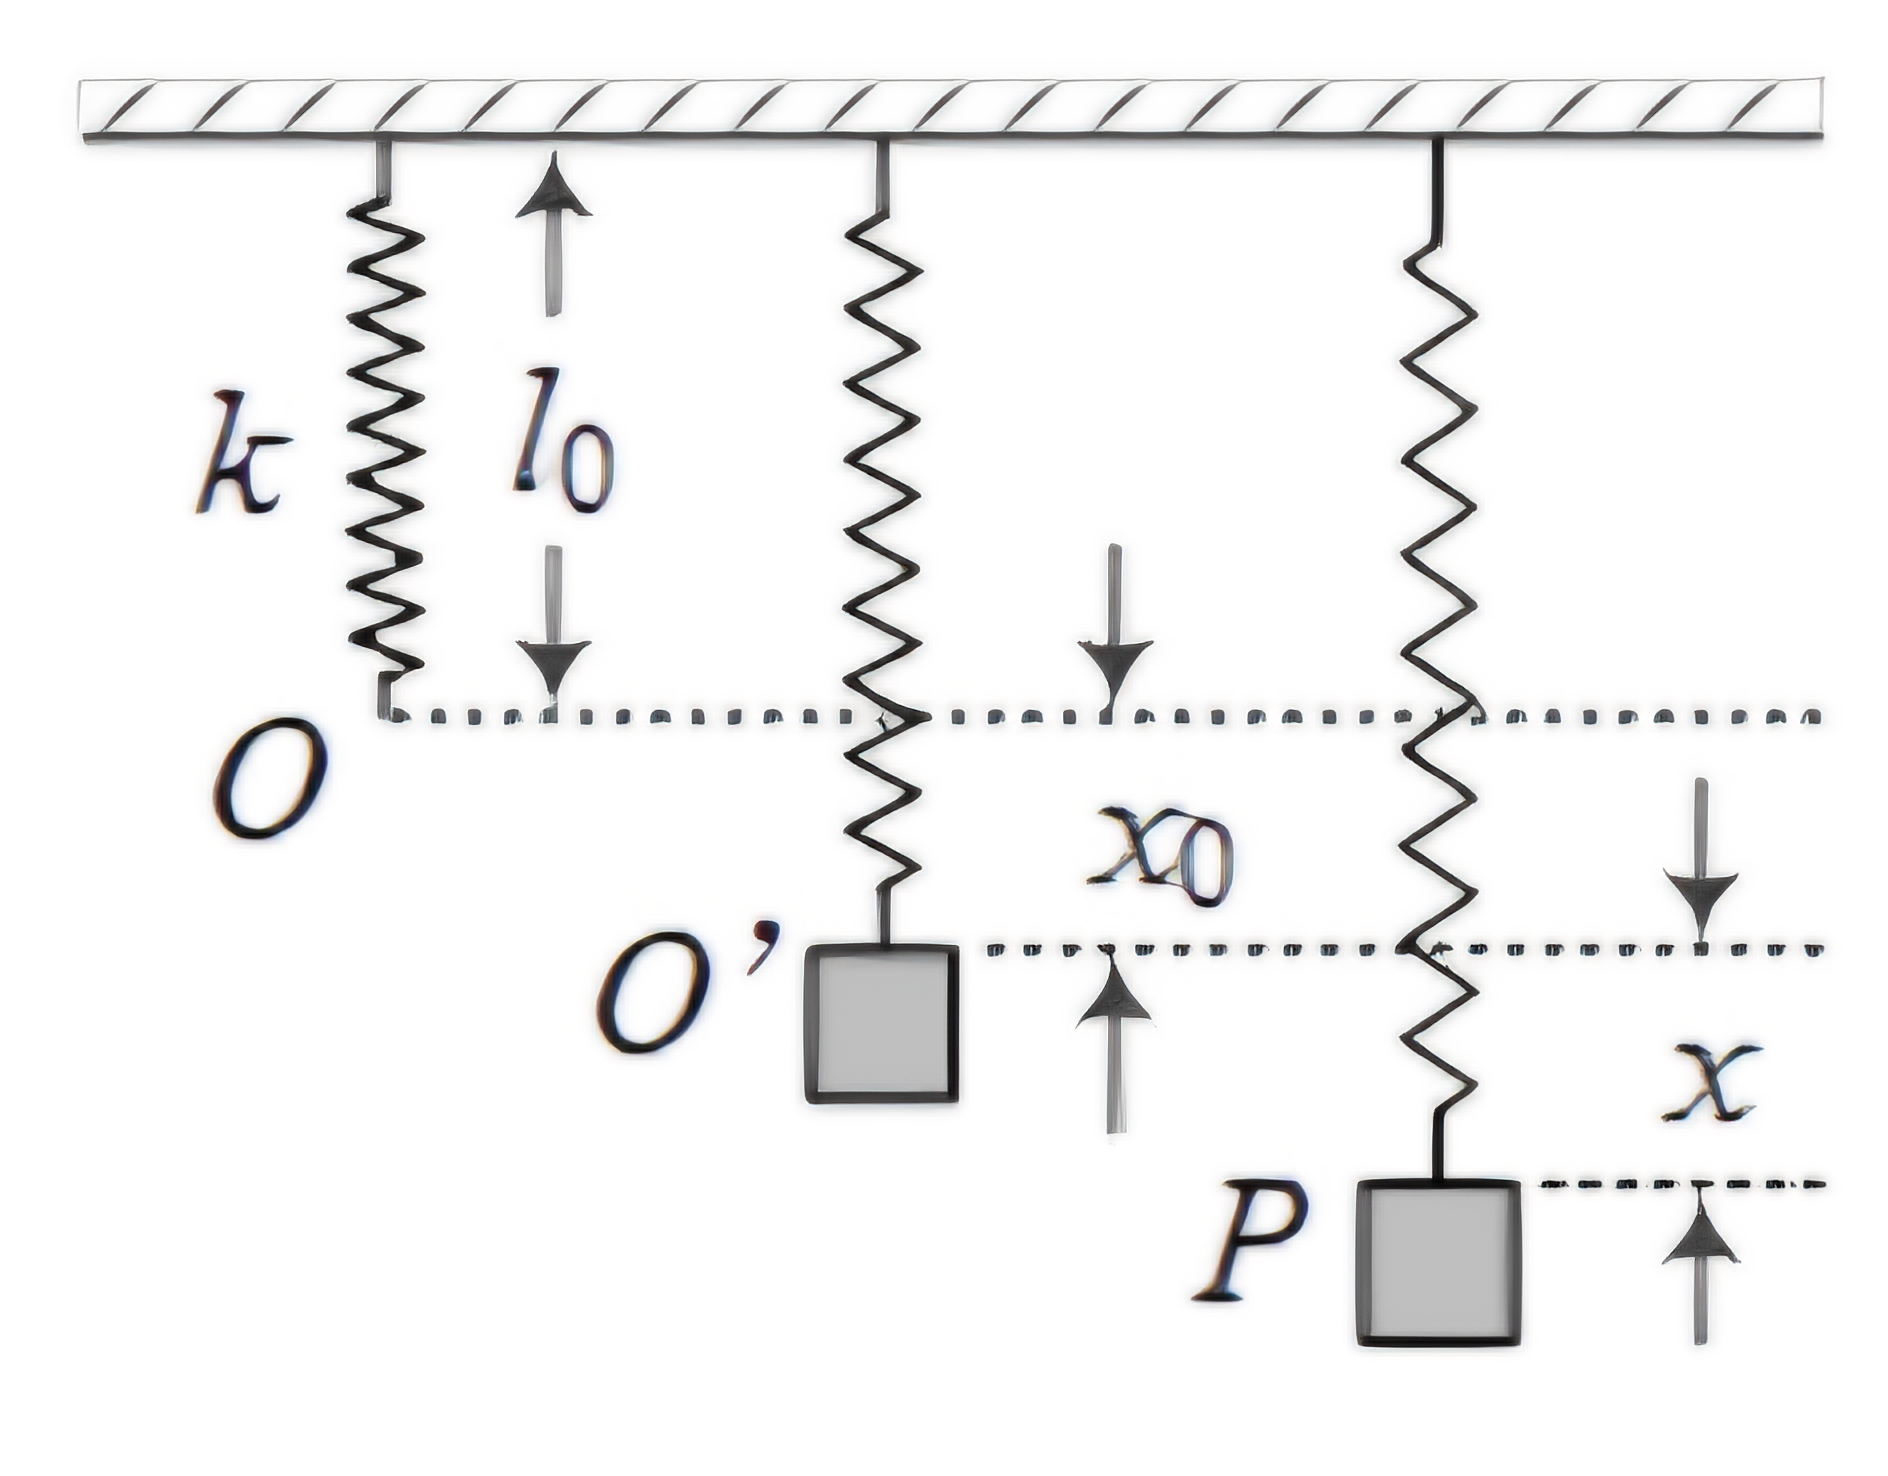
\includegraphics[scale=0.2]{"Chapter 04 images/pic2.png"}
        % \caption{}
        \label{pic4-2}
    \end{wrapfigure}

    \[
        \omega = \deriv{\theta}{t}
    \]

    \[
        \overrightarrow{v_i} = r_i \omega \overrightarrow{e}_t
    \]

    $$
        \overrightarrow{v}=\overrightarrow{\omega} \times \overrightarrow{r}_{\perp}=
        \overrightarrow{\omega} \times \overrightarrow{r}
    $$

    $$
        \alpha=\deriv{\omega}{t}=\frac{\rmd^2 \theta}{\rmd^2 t}
    $$

    于是

    \begin{equation}
        \overrightarrow{a}=r \alpha \overrightarrow{e}_{\mathrm{t}}+r \omega^2 \overrightarrow{e}_{\mathrm{n}}
    \end{equation}

\subsection{力矩}

\subsubsection{定义}

    用来描述力对刚体的转动的作用的物理量。

    \begin{wrapfigure}{r}{4cm}
        \centering
        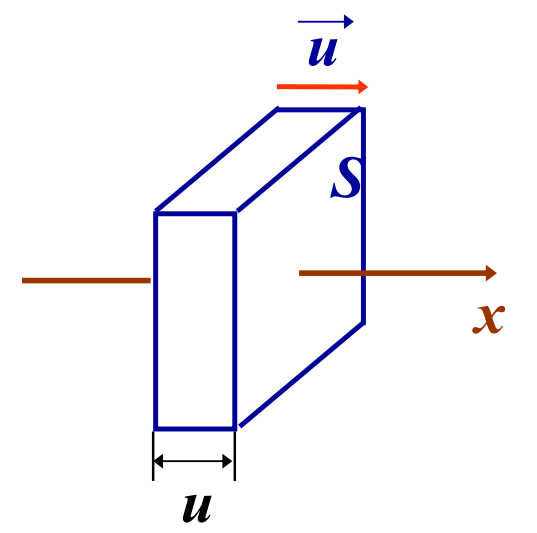
\includegraphics[scale=0.2]{"Chapter 04 images/pic3.png"}
        % \caption{}
        \label{pic4-3}
    \end{wrapfigure}

    刚体绕\(Oz\)轴旋转 , 力作用在刚体上点\(P\),且在转动平面内,为由点\(O\)到力的作用点\(P\)的径矢。
    \(\overrightarrow{F}\)对转轴\(z\)的力矩的定义:

    \begin{align}
        \overrightarrow{M} = \overrightarrow{r} \times \overrightarrow{F}
    \end{align}

    $$
        M = Fr\sin\theta = Fd \quad (d\text{为力臂})
    $$

\subsubsection{讨论}

    \begin{enumerate}
        \item 若力\(\overrightarrow{F}\)不在转动平面内,可将力分解为平行和垂直于转轴方向的两个分量;
        \item 合力矩等于各分力矩的矢量和;
        \item 刚体内作用力和反作用力的力矩相互抵消;
        \item 力矩的单位只能用\(\text{牛顿} \cdot \text{米}\),而不能用焦耳。
    \end{enumerate}

\section{转动定律、转动惯量}

\subsection{质点的转动惯量}

    单个质点\(m\)与转轴刚性连接

    \begin{wrapfigure}{r}{4cm}
        \centering
        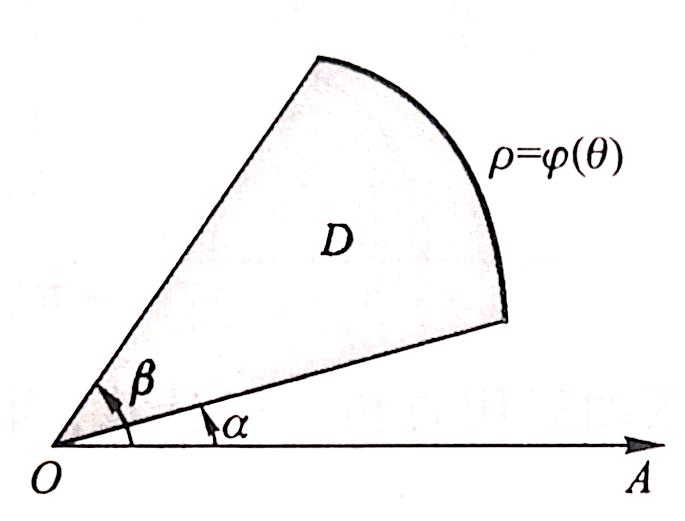
\includegraphics[scale=0.2]{"Chapter 04 images/pic4.png"}
        % \caption{}
        \label{pic4-4}
    \end{wrapfigure}

    $$
        F_{\mathrm{t}}=m a_{\mathrm{t}}=m r \alpha
    $$

    则

    \begin{equation}
        F_{\mathrm{t}}=m a_{\mathrm{t}}=m r \alpha
    \end{equation}

    \textbf{定义}

    \begin{align}
        J = mr^2
    \end{align}

    为质点\(m\)对\(O\)点的“转动惯量”。

    于是

    \begin{align}
        M = J \alpha
    \end{align}

\subsection{刚体的转动惯量}

    \begin{wrapfigure}{r}{4cm}
        \centering
        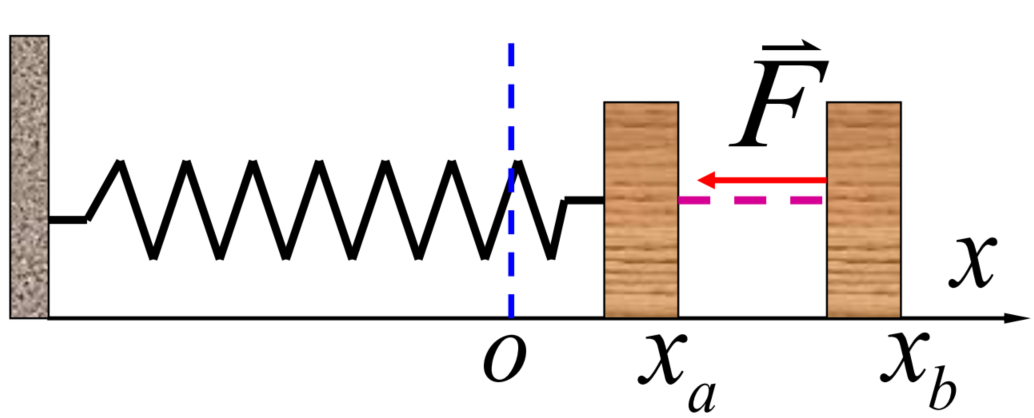
\includegraphics[scale=0.2]{"Chapter 04 images/pic5.png"}
        % \caption{}
        \label{pic4-5}
    \end{wrapfigure}

    质量元受外力\(\overrightarrow{F}_{\mathrm{e}j}\),内力\(\overrightarrow{F}_{\mathrm{i}j}\)

    则

    \begin{align*}
        M_{\mathrm{e} j}+M_{\mathrm{i} j}=\Delta m_j r_j^2 \alpha
    \end{align*}

    因为$M_{i j}=-M_{j i}$,所以

    $$
        \sum_j M_{i j}=0
    $$

    于是

    \begin{equation}
        \sum_j M_{\mathrm{e} j}=\left(\sum \Delta m_j r_j^2\right) \alpha
    \end{equation}

    \textbf{定义}

    \begin{align}
        J=\sum_j \Delta m_j r_j^2
    \end{align}

    为刚体对\(O\)点的“转动惯量”。

    积分形式即为

    \begin{equation}
        J=\int r^2 \mathrm{~d} m
    \end{equation}

\subsection{转动定律}

    \begin{align}
        M = J \alpha
    \end{align}

\subsubsection{讨论}

    \begin{enumerate}
        \item 若\(M=0\),则\(\alpha=0\),即\(\omega\)不变;
        \item \(\alpha \)与\(\frac{M}{J}\)成反比;
        \item \(M = J\alpha = J\deriv{\omega}{t}\);
        \item 转动惯量的单位为\(\mathrm{kg} \cdot \mathrm{m^2}\);
        \item 转动惯量的是对某一转轴而言的;
        \item 转动惯量是转动惯性的量度;
        \item 转动惯量具有可叠加性;
        \item 转动惯量与刚体的质量、质量的分布以及转轴的位置有关。
    \end{enumerate}

\end{document}
